% log sin and a primitive with its tangent; the potential along a line through theta.
% Source of the figure, typeset in the paper's own fonts (T1, Latin Modern, 11pt) at the paper's text
% width (6.5in), so \includegraphics does not rescale it. Illustrates CLH-2; it adds no assertion.
% Every coordinate and printed number is read from values that Lean evaluated (Conj43.crossEdges, the gaps, the primitive of log sin and the gradient);
% inputs: f-bar=(3,5,1,2,4), theta/pi=(0,0.1,0.7,0.3,0.8).
% SHA-256 (first 16 hex digits) of the output lines the values come from: prim 8a8931c181fce3de, line_e3 158868853e2d9d03.
% Real-valued quantities are floating-point values computed in Lean from the paper's formulas.
% Build: pdflatex <this file> && pdftocairo -svg <this file>.pdf <this file>.svg
\documentclass[11pt]{standalone}
\usepackage[T1]{fontenc}
\usepackage{lmodern}
\usepackage{amsmath,amssymb}
\usepackage{tikz}
\usetikzlibrary{arrows.meta,positioning,calc}

% the palette of the paper's other figures: blue solid for the first curve or strand, ochre dashed for the second
\definecolor{ink}{HTML}{233740}
\definecolor{muted}{HTML}{65757D}
\definecolor{pblue}{HTML}{0072B2}
\definecolor{qochre}{HTML}{B87827}

\tikzset{
  frm/.style={draw=muted, line width=0.5pt},
  axl/.style={draw=muted!70, line width=0.4pt},
  crvP/.style={draw=pblue, line width=1.1pt, line join=round},
  crvQ/.style={draw=qochre, line width=1.1pt, dash pattern=on 4pt off 1.6pt},
  drop/.style={draw=muted, line width=0.4pt, dash pattern=on 1pt off 1.4pt},
  dotQ/.style={circle, fill=qochre, draw=qochre, inner sep=0pt, minimum size=4.2pt},
  dotP/.style={circle, fill=pblue, draw=pblue, inner sep=0pt, minimum size=4.2pt},
  openQ/.style={circle, fill=white, draw=qochre, line width=0.8pt, inner sep=0pt, minimum size=4.2pt},
  lab/.style={font=\footnotesize, inner sep=1.5pt, text=ink},
  labm/.style={font=\small, inner sep=1.5pt, text=ink},
  labQ/.style={font=\footnotesize, inner sep=1.5pt, text=qochre},
  labP/.style={font=\footnotesize, inner sep=1.5pt, text=pblue},
  tick/.style={font=\footnotesize, inner sep=1.2pt, text=muted},
  vtx/.style={circle, draw=ink, fill=white, line width=0.6pt, inner sep=0pt, minimum size=15pt, font=\small, text=ink},
  arrP/.style={pblue, line width=1.0pt, -{Stealth[length=5pt,width=4.2pt]}},
}

\begin{document}
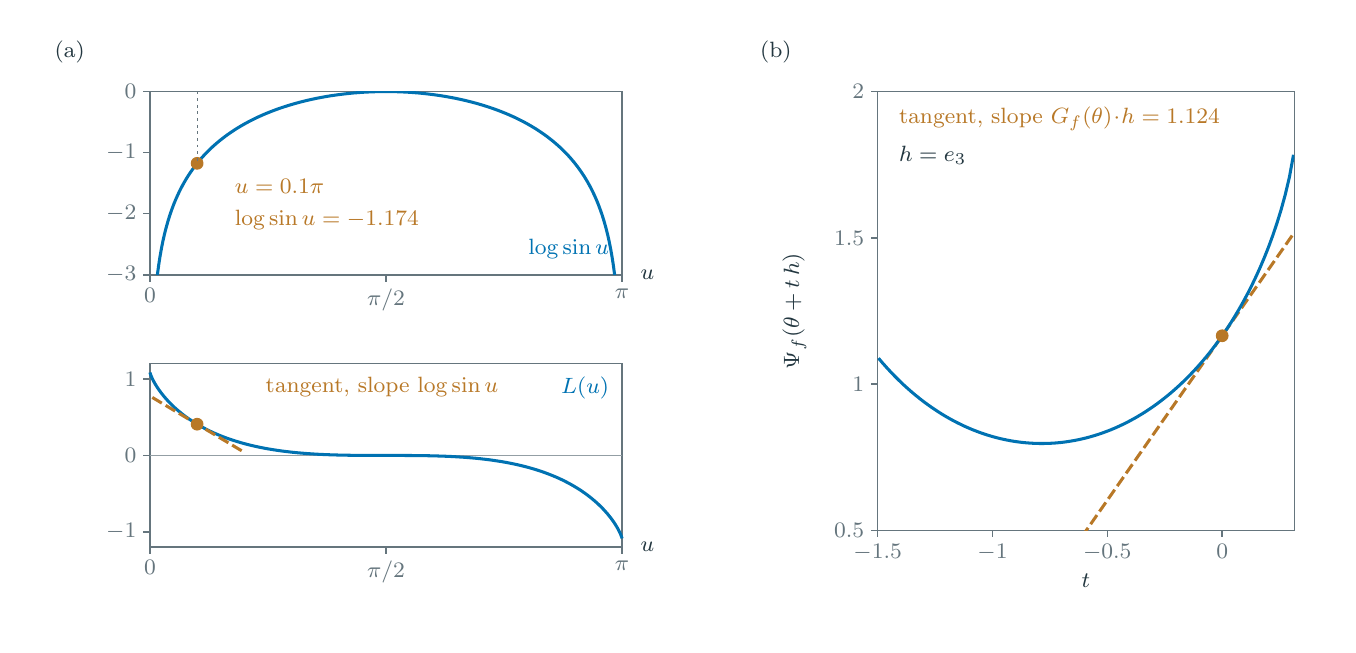
\begin{tikzpicture}[x=1bp,y=1bp]
\useasboundingbox (0,0) rectangle (468.005,215.0025);
\node[lab, anchor=north west] at (8.00,212.00) {(a)};
% map P1 44.0000 192.0000 170.0000 22.0000
\draw[frm] (44.00,126.00) rectangle (214.00,192.00);
\draw[frm] (44.00,126.00) -- (44.00,123.50);
\node[tick, anchor=north] at (44.00,122.50) {$0$};
\draw[frm] (129.00,126.00) -- (129.00,123.50);
\node[tick, anchor=north] at (129.00,122.50) {$\pi/2$};
\draw[frm] (214.00,126.00) -- (214.00,123.50);
\node[tick, anchor=north] at (214.00,122.50) {$\pi$};
\draw[frm] (44.00,126.00) -- (41.50,126.00);
\node[tick, anchor=east] at (40.50,126.00) {$-3$};
\draw[frm] (44.00,148.00) -- (41.50,148.00);
\node[tick, anchor=east] at (40.50,148.00) {$-2$};
\draw[frm] (44.00,170.00) -- (41.50,170.00);
\node[tick, anchor=east] at (40.50,170.00) {$-1$};
\draw[frm] (44.00,192.00) -- (41.50,192.00);
\node[tick, anchor=east] at (40.50,192.00) {$0$};
\begin{scope}\clip (44.00,126.00) rectangle (214.00,192.00);
\draw[crvP] (44.02,13.75) -- (44.07,44.24) -- (44.15,62.08) -- (44.26,74.73) -- (44.41,84.54) -- (44.59,92.56) -- (44.80,99.33) -- (45.05,105.19) -- (45.32,110.36) -- (45.63,114.99) -- (45.97,119.16) -- (46.35,122.97) -- (46.75,126.47) -- (47.19,129.71) -- (47.66,132.72) -- (48.16,135.54) -- (48.69,138.18) -- (49.25,140.66) -- (49.85,143.00) -- (50.47,145.22) -- (51.12,147.33) -- (51.81,149.33) -- (52.52,151.24) -- (53.26,153.06) -- (54.04,154.81) -- (54.84,156.48) -- (55.67,158.08) -- (56.53,159.61) -- (57.41,161.09) -- (58.33,162.50) -- (59.27,163.87) -- (60.23,165.18) -- (61.23,166.45) -- (62.25,167.67) -- (63.29,168.84) -- (64.37,169.98) -- (65.46,171.07) -- (66.58,172.13) -- (67.73,173.15) -- (68.90,174.14) -- (70.09,175.09) -- (71.30,176.01) -- (72.54,176.89) -- (73.80,177.75) -- (75.08,178.58) -- (76.38,179.37) -- (77.70,180.14) -- (79.04,180.88) -- (80.40,181.59) -- (81.78,182.28) -- (83.17,182.94) -- (84.59,183.57) -- (86.02,184.18) -- (87.47,184.76) -- (88.93,185.32) -- (90.41,185.86) -- (91.91,186.37) -- (93.41,186.85) -- (94.94,187.32) -- (96.47,187.76) -- (98.02,188.18) -- (99.58,188.57) -- (101.15,188.95) -- (102.73,189.30) -- (104.33,189.63) -- (105.93,189.94) -- (107.54,190.22) -- (109.16,190.49) -- (110.78,190.73) -- (112.42,190.95) -- (114.06,191.15) -- (115.70,191.33) -- (117.35,191.49) -- (119.01,191.62) -- (120.67,191.74) -- (122.33,191.83) -- (124.00,191.91) -- (125.66,191.96) -- (127.33,191.99) -- (129.00,192.00) -- (130.67,191.99) -- (132.34,191.96) -- (134.00,191.91) -- (135.67,191.83) -- (137.33,191.74) -- (138.99,191.62) -- (140.65,191.49) -- (142.30,191.33) -- (143.94,191.15) -- (145.58,190.95) -- (147.22,190.73) -- (148.84,190.49) -- (150.46,190.22) -- (152.07,189.94) -- (153.67,189.63) -- (155.27,189.30) -- (156.85,188.95) -- (158.42,188.57) -- (159.98,188.18) -- (161.53,187.76) -- (163.06,187.32) -- (164.59,186.85) -- (166.09,186.37) -- (167.59,185.86) -- (169.07,185.32) -- (170.53,184.76) -- (171.98,184.18) -- (173.41,183.57) -- (174.83,182.94) -- (176.22,182.28) -- (177.60,181.59) -- (178.96,180.88) -- (180.30,180.14) -- (181.62,179.37) -- (182.92,178.58) -- (184.20,177.75) -- (185.46,176.89) -- (186.70,176.01) -- (187.91,175.09) -- (189.10,174.14) -- (190.27,173.15) -- (191.42,172.13) -- (192.54,171.07) -- (193.63,169.98) -- (194.71,168.84) -- (195.75,167.67) -- (196.77,166.45) -- (197.77,165.18) -- (198.73,163.87) -- (199.67,162.50) -- (200.59,161.09) -- (201.47,159.61) -- (202.33,158.08) -- (203.16,156.48) -- (203.96,154.81) -- (204.74,153.06) -- (205.48,151.24) -- (206.19,149.33) -- (206.88,147.33) -- (207.53,145.22) -- (208.15,143.00) -- (208.75,140.66) -- (209.31,138.18) -- (209.84,135.54) -- (210.34,132.72) -- (210.81,129.71) -- (211.25,126.47) -- (211.65,122.97) -- (212.03,119.16) -- (212.37,114.99) -- (212.68,110.36) -- (212.95,105.19) -- (213.20,99.33) -- (213.41,92.56) -- (213.59,84.54) -- (213.74,74.73) -- (213.85,62.08) -- (213.93,44.24) -- (213.98,13.75); %curve P1 logsin
\end{scope}
\node[dotQ] at (61.00,166.16) {}; %mark P1 logsin 0
\draw[drop] (61.00,192.00) -- (61.00,166.16);
\node[labP, anchor=south east] at (211.00,130.00) {$\log\sin u$};
\node[lab, anchor=west] at (219.00,126.00) {$u$};
\node[labQ, anchor=west] at (72.90,157.90) {$u=0.1\pi$}; %val u 0 0.1
\node[labQ, anchor=west] at (72.90,145.90) {$\log\sin u=-1.174$}; %val slope 0 -1.174
% map P2 44.0000 61.0000 170.0000 27.5000
\draw[frm] (44.00,28.00) rectangle (214.00,94.00);
\draw[frm] (44.00,28.00) -- (44.00,25.50);
\node[tick, anchor=north] at (44.00,24.50) {$0$};
\draw[frm] (129.00,28.00) -- (129.00,25.50);
\node[tick, anchor=north] at (129.00,24.50) {$\pi/2$};
\draw[frm] (214.00,28.00) -- (214.00,25.50);
\node[tick, anchor=north] at (214.00,24.50) {$\pi$};
\draw[frm] (44.00,33.50) -- (41.50,33.50);
\node[tick, anchor=east] at (40.50,33.50) {$-1$};
\draw[frm] (44.00,61.00) -- (41.50,61.00);
\node[tick, anchor=east] at (40.50,61.00) {$0$};
\draw[frm] (44.00,88.50) -- (41.50,88.50);
\node[tick, anchor=east] at (40.50,88.50) {$1$};
\draw[axl] (44.00,61.00) -- (214.00,61.00);
\draw[crvP] (44.02,90.88) -- (44.07,90.69) -- (44.15,90.43) -- (44.26,90.10) -- (44.41,89.72) -- (44.59,89.29) -- (44.80,88.82) -- (45.05,88.31) -- (45.32,87.77) -- (45.63,87.21) -- (45.97,86.62) -- (46.35,86.00) -- (46.75,85.37) -- (47.19,84.73) -- (47.66,84.07) -- (48.16,83.40) -- (48.69,82.73) -- (49.25,82.04) -- (49.85,81.36) -- (50.47,80.67) -- (51.12,79.98) -- (51.81,79.29) -- (52.52,78.60) -- (53.26,77.92) -- (54.04,77.24) -- (54.84,76.57) -- (55.67,75.90) -- (56.53,75.24) -- (57.41,74.60) -- (58.33,73.96) -- (59.27,73.33) -- (60.23,72.72) -- (61.23,72.12) -- (62.25,71.53) -- (63.29,70.96) -- (64.37,70.40) -- (65.46,69.85) -- (66.58,69.32) -- (67.73,68.81) -- (68.90,68.32) -- (70.09,67.84) -- (71.30,67.38) -- (72.54,66.93) -- (73.80,66.51) -- (75.08,66.10) -- (76.38,65.71) -- (77.70,65.33) -- (79.04,64.98) -- (80.40,64.64) -- (81.78,64.32) -- (83.17,64.02) -- (84.59,63.73) -- (86.02,63.46) -- (87.47,63.21) -- (88.93,62.98) -- (90.41,62.76) -- (91.91,62.55) -- (93.41,62.37) -- (94.94,62.19) -- (96.47,62.03) -- (98.02,61.89) -- (99.58,61.76) -- (101.15,61.64) -- (102.73,61.54) -- (104.33,61.44) -- (105.93,61.36) -- (107.54,61.29) -- (109.16,61.23) -- (110.78,61.18) -- (112.42,61.13) -- (114.06,61.10) -- (115.70,61.07) -- (117.35,61.05) -- (119.01,61.03) -- (120.67,61.02) -- (122.33,61.01) -- (124.00,61.00) -- (125.66,61.00) -- (127.33,61.00) -- (129.00,61.00) -- (130.67,61.00) -- (132.34,61.00) -- (134.00,61.00) -- (135.67,60.99) -- (137.33,60.98) -- (138.99,60.97) -- (140.65,60.95) -- (142.30,60.93) -- (143.94,60.90) -- (145.58,60.87) -- (147.22,60.82) -- (148.84,60.77) -- (150.46,60.71) -- (152.07,60.64) -- (153.67,60.56) -- (155.27,60.46) -- (156.85,60.36) -- (158.42,60.24) -- (159.98,60.11) -- (161.53,59.97) -- (163.06,59.81) -- (164.59,59.63) -- (166.09,59.45) -- (167.59,59.24) -- (169.07,59.02) -- (170.53,58.79) -- (171.98,58.54) -- (173.41,58.27) -- (174.83,57.98) -- (176.22,57.68) -- (177.60,57.36) -- (178.96,57.02) -- (180.30,56.67) -- (181.62,56.29) -- (182.92,55.90) -- (184.20,55.49) -- (185.46,55.07) -- (186.70,54.62) -- (187.91,54.16) -- (189.10,53.68) -- (190.27,53.19) -- (191.42,52.68) -- (192.54,52.15) -- (193.63,51.60) -- (194.71,51.04) -- (195.75,50.47) -- (196.77,49.88) -- (197.77,49.28) -- (198.73,48.67) -- (199.67,48.04) -- (200.59,47.40) -- (201.47,46.76) -- (202.33,46.10) -- (203.16,45.43) -- (203.96,44.76) -- (204.74,44.08) -- (205.48,43.40) -- (206.19,42.71) -- (206.88,42.02) -- (207.53,41.33) -- (208.15,40.64) -- (208.75,39.96) -- (209.31,39.27) -- (209.84,38.60) -- (210.34,37.93) -- (210.81,37.27) -- (211.25,36.63) -- (211.65,36.00) -- (212.03,35.38) -- (212.37,34.79) -- (212.68,34.23) -- (212.95,33.69) -- (213.20,33.18) -- (213.41,32.71) -- (213.59,32.28) -- (213.74,31.90) -- (213.85,31.57) -- (213.93,31.31) -- (213.98,31.12); %curve P2 L
\draw[crvQ] (44.87,81.88) -- (77.13,62.63); %curve P2 tangent
\node[dotQ] at (61.00,72.25) {}; %mark P2 L 0
\node[labP, anchor=north east] at (211.00,91.00) {$L(u)$};
\node[labQ, anchor=north west] at (84.00,91.00) {tangent, slope $\log\sin u$};
\node[lab, anchor=west] at (219.00,28.00) {$u$};
\node[lab, anchor=north west] at (262.00,212.00) {(b)};
% map P3 430.0244 -18.6667 82.6829 105.3333
\draw[frm] (306.00,34.00) rectangle (456.00,192.00);
\draw[frm] (306.00,34.00) -- (306.00,31.50);
\node[tick, anchor=north] at (306.00,30.50) {$-1.5$};
\draw[frm] (347.34,34.00) -- (347.34,31.50);
\node[tick, anchor=north] at (347.34,30.50) {$-1$};
\draw[frm] (388.68,34.00) -- (388.68,31.50);
\node[tick, anchor=north] at (388.68,30.50) {$-0.5$};
\draw[frm] (430.02,34.00) -- (430.02,31.50);
\node[tick, anchor=north] at (430.02,30.50) {$0$};
\draw[frm] (306.00,34.00) -- (303.50,34.00);
\node[tick, anchor=east] at (302.50,34.00) {$0.5$};
\draw[frm] (306.00,86.67) -- (303.50,86.67);
\node[tick, anchor=east] at (302.50,86.67) {$1$};
\draw[frm] (306.00,139.33) -- (303.50,139.33);
\node[tick, anchor=east] at (302.50,139.33) {$1.5$};
\draw[frm] (306.00,192.00) -- (303.50,192.00);
\node[tick, anchor=east] at (302.50,192.00) {$2$};
\begin{scope}\clip (306.00,34.00) rectangle (456.00,192.00);
\draw[crvQ] (306.00,-73.53) -- (456.00,141.29); %curve P3 tangent
\draw[crvP] (306.30,96.02) -- (307.79,94.26) -- (309.29,92.58) -- (310.78,90.97) -- (312.28,89.42) -- (313.77,87.94) -- (315.26,86.51) -- (316.76,85.15) -- (318.25,83.84) -- (319.75,82.59) -- (321.24,81.39) -- (322.73,80.24) -- (324.23,79.15) -- (325.72,78.10) -- (327.22,77.10) -- (328.71,76.14) -- (330.20,75.23) -- (331.70,74.37) -- (333.19,73.55) -- (334.69,72.77) -- (336.18,72.04) -- (337.67,71.34) -- (339.17,70.69) -- (340.66,70.07) -- (342.16,69.50) -- (343.65,68.96) -- (345.14,68.46) -- (346.64,68.00) -- (348.13,67.58) -- (349.63,67.19) -- (351.12,66.84) -- (352.61,66.53) -- (354.11,66.25) -- (355.60,66.01) -- (357.10,65.80) -- (358.59,65.63) -- (360.08,65.50) -- (361.58,65.40) -- (363.07,65.33) -- (364.57,65.30) -- (366.06,65.31) -- (367.55,65.35) -- (369.05,65.42) -- (370.54,65.53) -- (372.04,65.68) -- (373.53,65.86) -- (375.02,66.08) -- (376.52,66.33) -- (378.01,66.62) -- (379.51,66.94) -- (381.00,67.30) -- (382.49,67.70) -- (383.99,68.14) -- (385.48,68.61) -- (386.98,69.12) -- (388.47,69.67) -- (389.96,70.25) -- (391.46,70.88) -- (392.95,71.55) -- (394.45,72.26) -- (395.94,73.00) -- (397.43,73.80) -- (398.93,74.63) -- (400.42,75.51) -- (401.92,76.43) -- (403.41,77.40) -- (404.90,78.41) -- (406.40,79.47) -- (407.89,80.59) -- (409.39,81.75) -- (410.88,82.96) -- (412.37,84.23) -- (413.87,85.56) -- (415.36,86.94) -- (416.86,88.38) -- (418.35,89.88) -- (419.84,91.45) -- (421.34,93.09) -- (422.83,94.79) -- (424.33,96.57) -- (425.82,98.42) -- (427.31,100.36) -- (428.81,102.38) -- (430.30,104.49) -- (431.80,106.69) -- (433.29,109.00) -- (434.78,111.42) -- (436.28,113.96) -- (437.77,116.62) -- (439.27,119.42) -- (440.76,122.38) -- (442.25,125.50) -- (443.75,128.81) -- (445.24,132.33) -- (446.74,136.10) -- (448.23,140.16) -- (449.72,144.56) -- (451.22,149.40) -- (452.71,154.82) -- (454.21,161.11) -- (455.70,169.24); %curve P3 Psi
\end{scope}
\node[dotQ] at (430.02,104.09) {}; %mark P3 Psi 0
\node[lab, anchor=north] at (381.00,20.00) {$t$};
\node[lab, anchor=south, rotate=90] at (282.00,113.00) {$\Psi_f(\theta+t\,h)$};
\node[labQ, anchor=north west] at (312.00,188.00) {tangent, slope $G_f(\theta)\!\cdot\!h=1.124$}; %val slope 1 1.124
\node[lab, anchor=north west] at (312.00,174.00) {$h=e_3$};
\end{tikzpicture}
\end{document}
